\documentclass[class=article, crop=false]{standalone}
\usepackage{graphicx}
\graphicspath{{../Figures}}
\setkeys{Gin}{width=\textwidth}

\usepackage{caption}
\usepackage{subcaption}
\usepackage[subsection]{placeins}

\begin{document}

\section{USV position}
\FloatBarrier
\subsection{Uncontrolled}
\begin{figure}
    \centering
    \begin{subfigure}[b]{0.48\textwidth}
        \centering
        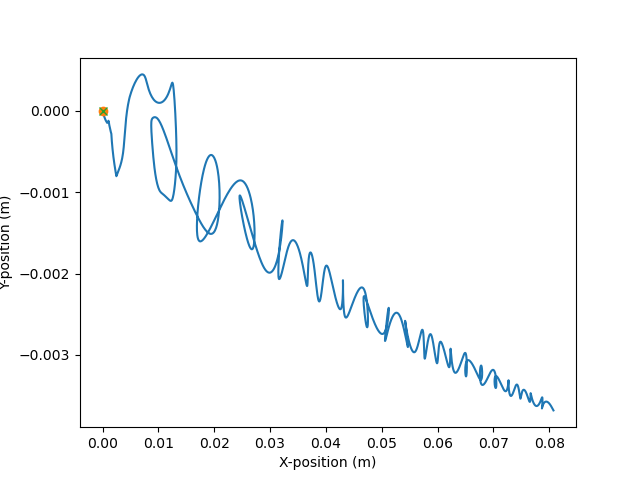
\includegraphics{scenario1/rov-0m/0.0m/usv_position_uncontrolled}
        \caption{0m}
        \label{}
    \end{subfigure}
    \hfill
    \begin{subfigure}[b]{0.48\textwidth}
        \centering
        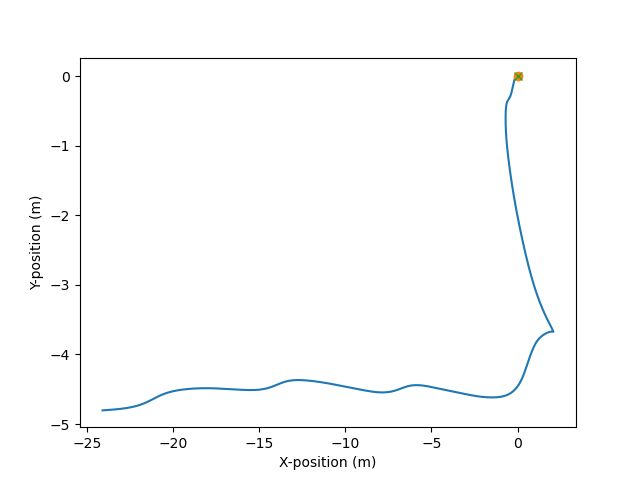
\includegraphics{scenario1/rov-0m/0.5m/usv_position_uncontrolled}
        \caption{0.5m}
        \label{}
    \end{subfigure}
    \vfill
    \begin{subfigure}[b]{0.48\textwidth}
        \centering
        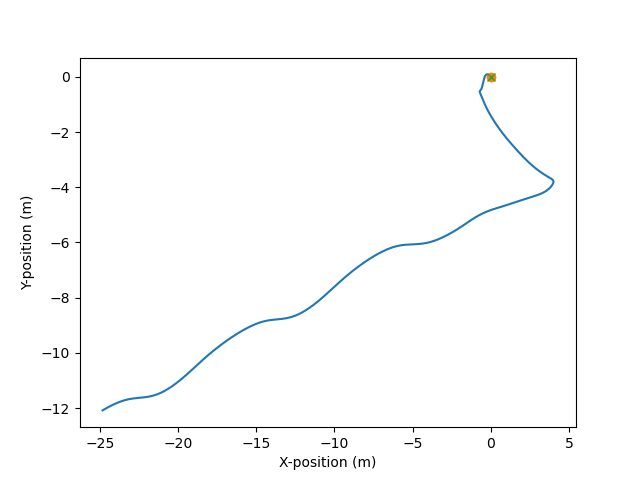
\includegraphics{scenario1/rov-0m/1.0m/usv_position_uncontrolled}
        \caption{1m}
        \label{}
    \end{subfigure}
    \hfill
    \begin{subfigure}[b]{0.48\textwidth}
        \centering
        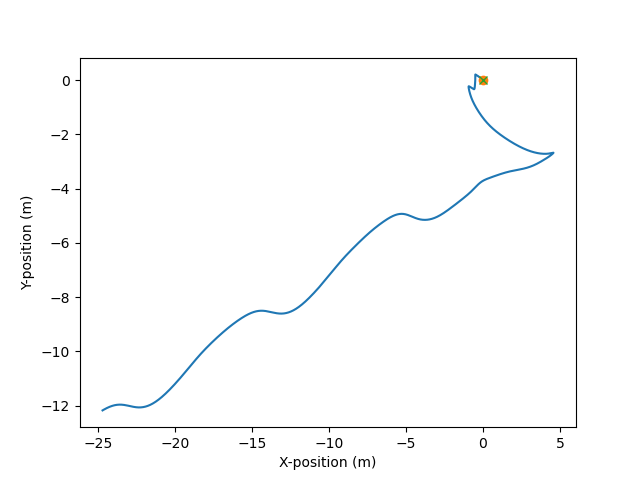
\includegraphics{scenario1/rov-0m/1.5m/usv_position_uncontrolled}
        \caption{1.5m}
        \label{}
    \end{subfigure}
    \vfill
    \begin{subfigure}[b]{0.48\textwidth}
        \centering
        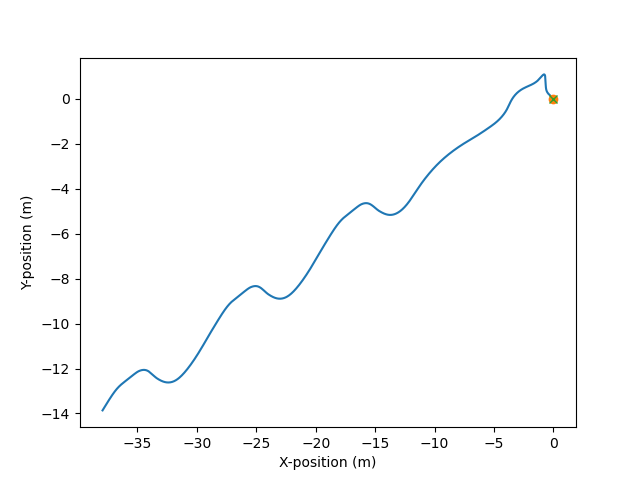
\includegraphics{scenario1/rov-0m/2.0m/usv_position_uncontrolled}
        \caption{2m}
        \label{}
    \end{subfigure}

    \caption{USV position without control at different wave heights, ROV at 0m}
\end{figure}

\begin{figure}
    \centering
    \begin{subfigure}[b]{0.48\textwidth}
        \centering
        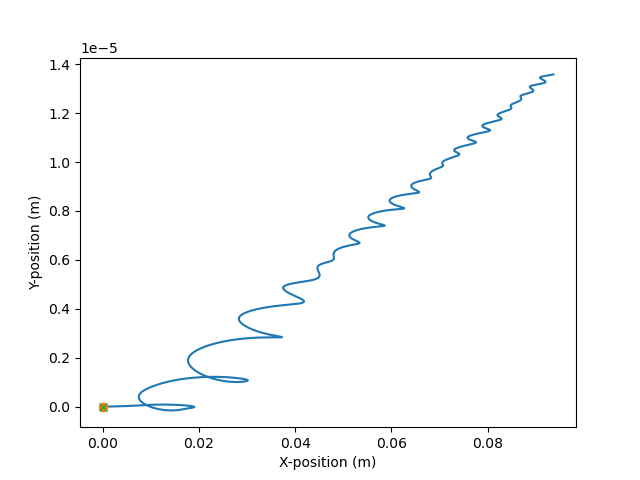
\includegraphics{scenario1/rov-50m/0.0m/usv_position_uncontrolled}
        \caption{0m}
        \label{}
    \end{subfigure}
    \hfill
    \begin{subfigure}[b]{0.48\textwidth}
        \centering
        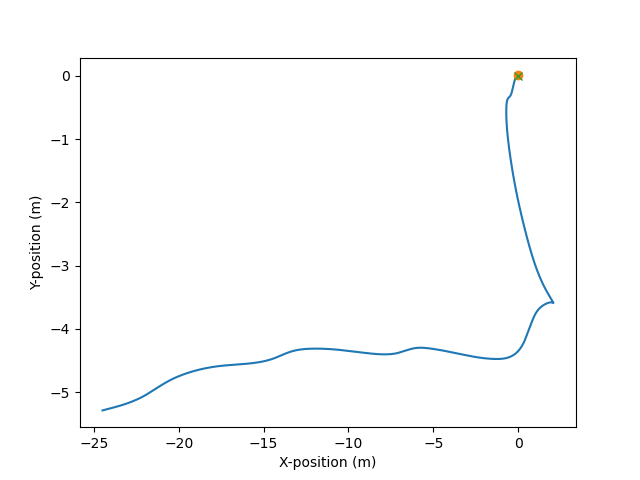
\includegraphics{scenario1/rov-50m/0.5m/usv_position_uncontrolled}
        \caption{0.5m}
        \label{}
    \end{subfigure}
    \vfill
    \begin{subfigure}[b]{0.48\textwidth}
        \centering
        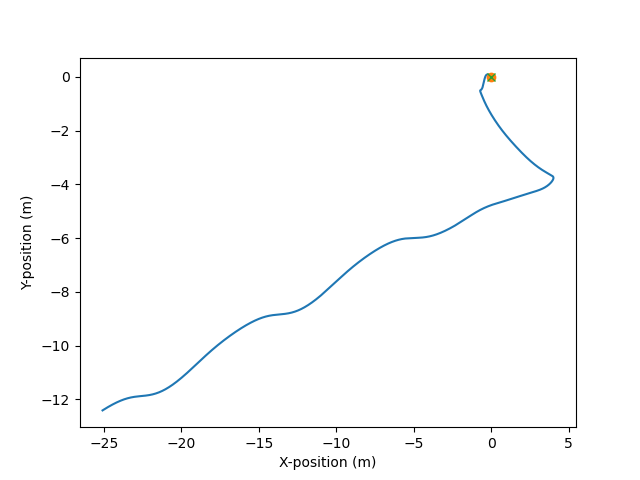
\includegraphics{scenario1/rov-50m/1.0m/usv_position_uncontrolled}
        \caption{1m}
        \label{}
    \end{subfigure}
    \hfill
    \begin{subfigure}[b]{0.48\textwidth}
        \centering
        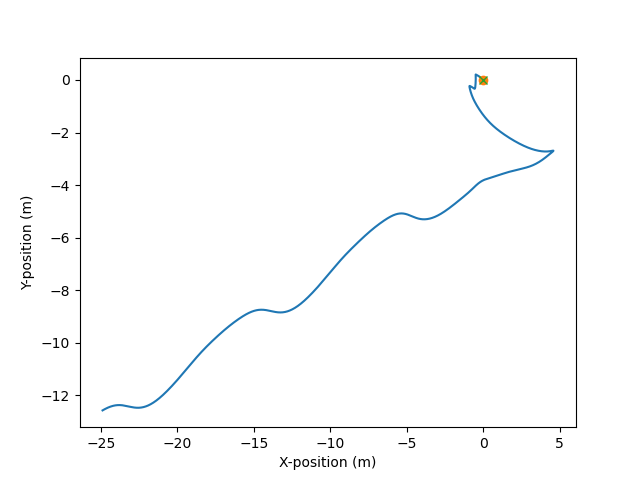
\includegraphics{scenario1/rov-50m/1.5m/usv_position_uncontrolled}
        \caption{1.5m}
        \label{}
    \end{subfigure}
    \vfill
    \begin{subfigure}[b]{0.48\textwidth}
        \centering
        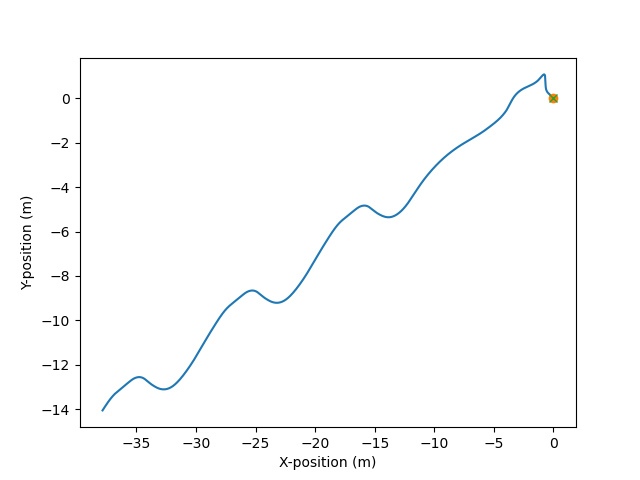
\includegraphics{scenario1/rov-50m/2.0m/usv_position_uncontrolled}
        \caption{2m}
        \label{}
    \end{subfigure}

    \caption{USV position without control at different wave heights, ROV at 50m}
\end{figure}

\begin{figure}
    \centering
    \begin{subfigure}[b]{0.48\textwidth}
        \centering
        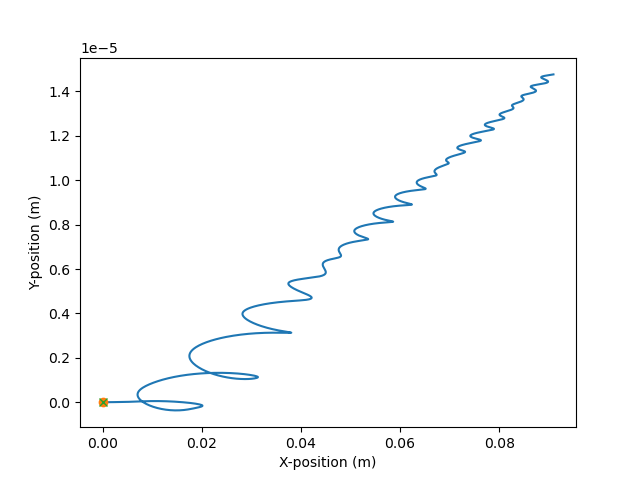
\includegraphics{scenario1/rov-100m/0.0m/usv_position_uncontrolled}
        \caption{0m}
        \label{}
    \end{subfigure}
    \hfill
    \begin{subfigure}[b]{0.48\textwidth}
        \centering
        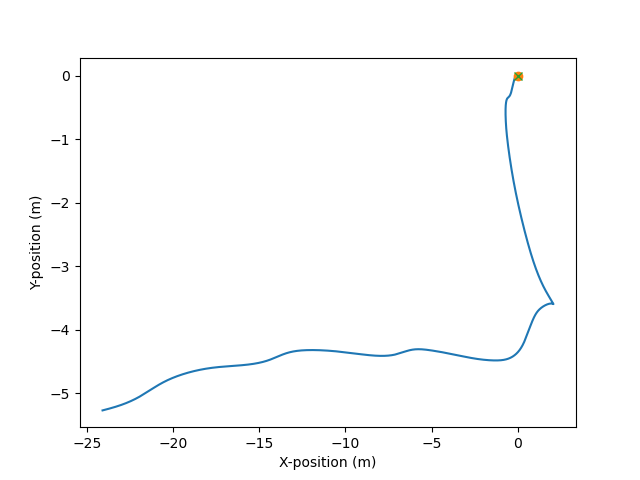
\includegraphics{scenario1/rov-100m/0.5m/usv_position_uncontrolled}
        \caption{0.5m}
        \label{}
    \end{subfigure}
    \vfill
    \begin{subfigure}[b]{0.48\textwidth}
        \centering
        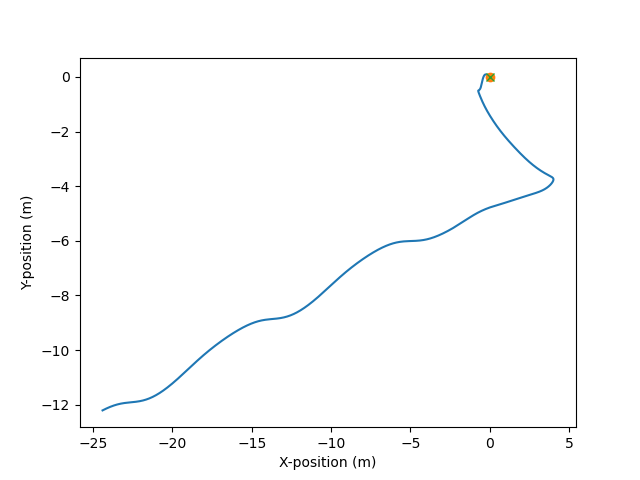
\includegraphics{scenario1/rov-100m/1.0m/usv_position_uncontrolled}
        \caption{1m}
        \label{}
    \end{subfigure}
    \hfill
    \begin{subfigure}[b]{0.48\textwidth}
        \centering
        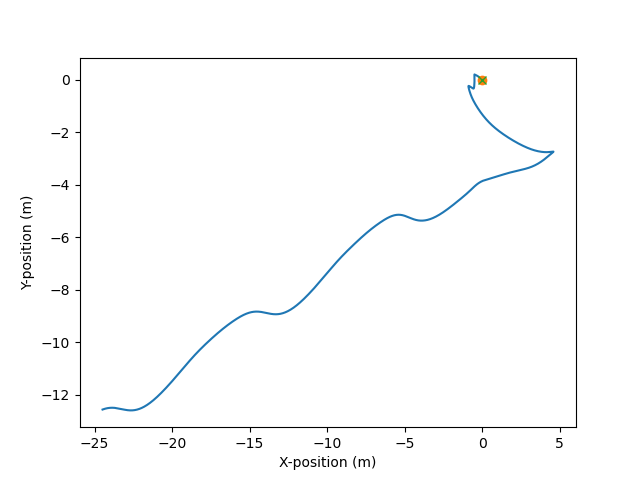
\includegraphics{scenario1/rov-100m/1.5m/usv_position_uncontrolled}
        \caption{1.5m}
        \label{}
    \end{subfigure}
    \vfill
    \begin{subfigure}[b]{0.48\textwidth}
        \centering
        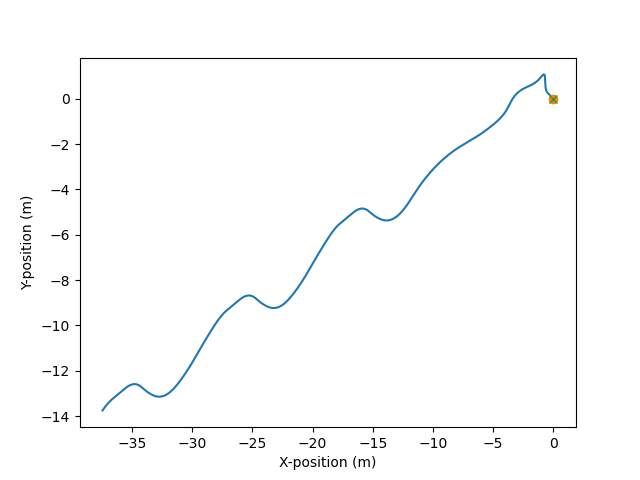
\includegraphics{scenario1/rov-100m/2.0m/usv_position_uncontrolled}
        \caption{2m}
        \label{}
    \end{subfigure}

    \caption{USV position without control at different wave heights, ROV at 100m}
\end{figure}
\FloatBarrier
\subsection{Controlled}
\begin{figure}
    \centering
    \begin{subfigure}[b]{0.48\textwidth}
        \centering
        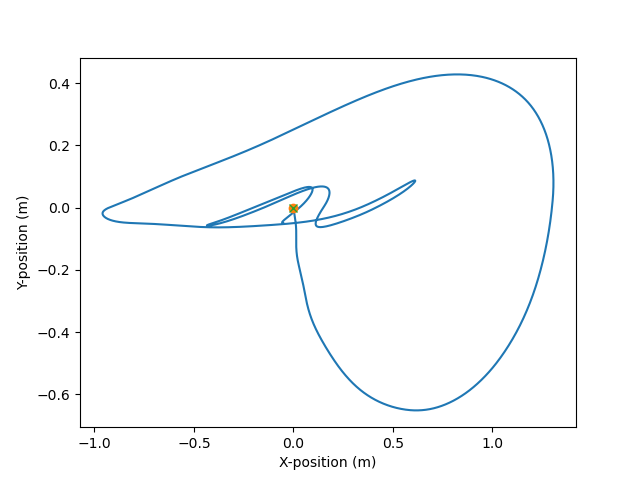
\includegraphics{scenario1/rov-0m/0.0m/usv_position_controlled}
        \caption{0m}
        \label{}
    \end{subfigure}
    \hfill
    \begin{subfigure}[b]{0.48\textwidth}
        \centering
        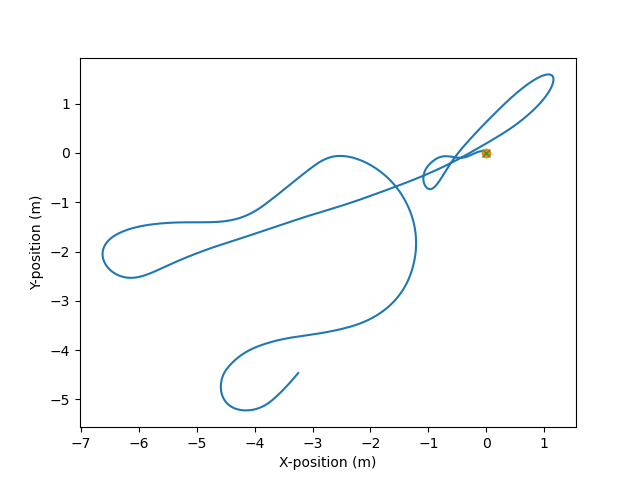
\includegraphics{scenario1/rov-0m/0.5m/usv_position_controlled}
        \caption{0.5m}
        \label{}
    \end{subfigure}
    \vfill
    \begin{subfigure}[b]{0.48\textwidth}
        \centering
        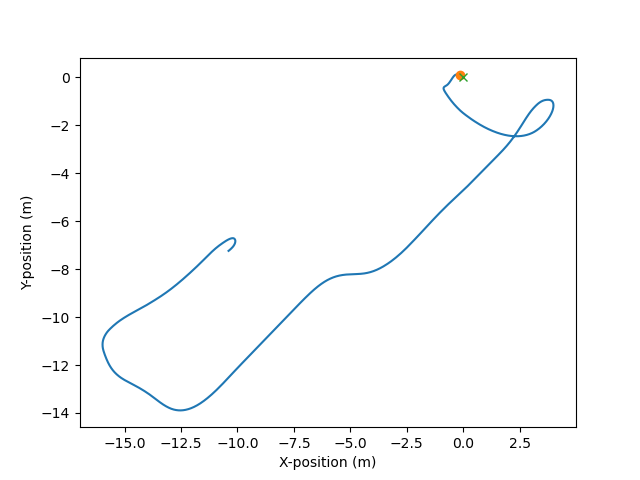
\includegraphics{scenario1/rov-0m/1.0m/usv_position_controlled}
        \caption{1m}
        \label{}
    \end{subfigure}
    \hfill
    \begin{subfigure}[b]{0.48\textwidth}
        \centering
        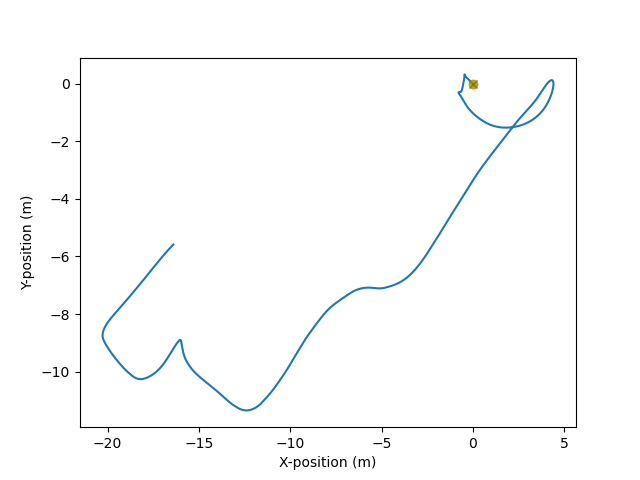
\includegraphics{scenario1/rov-0m/1.5m/usv_position_controlled}
        \caption{1.5m}
        \label{}
    \end{subfigure}
    \vfill
    \begin{subfigure}[b]{0.48\textwidth}
        \centering
        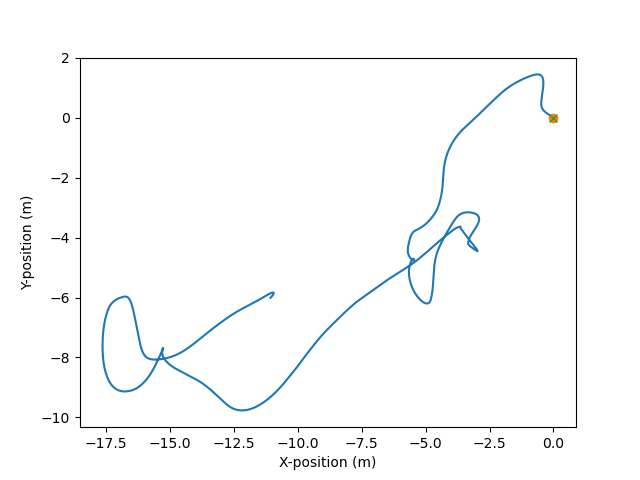
\includegraphics{scenario1/rov-0m/2.0m/usv_position_controlled}
        \caption{2m}
        \label{}
    \end{subfigure}

    \caption{USV position with control at different wave heights, ROV at 0m}
\end{figure}

\begin{figure}
    \centering
    \begin{subfigure}[b]{0.48\textwidth}
        \centering
        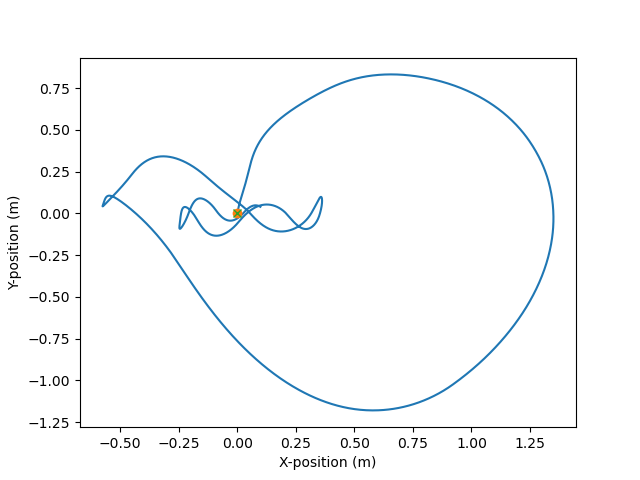
\includegraphics{scenario1/rov-50m/0.0m/usv_position_controlled}
        \caption{0m}
        \label{}
    \end{subfigure}
    \hfill
    \begin{subfigure}[b]{0.48\textwidth}
        \centering
        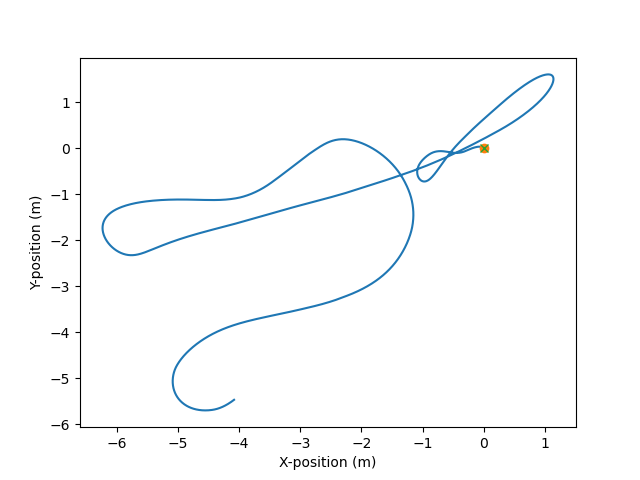
\includegraphics{scenario1/rov-50m/0.5m/usv_position_controlled}
        \caption{0.5m}
        \label{}
    \end{subfigure}
    \vfill
    \begin{subfigure}[b]{0.48\textwidth}
        \centering
        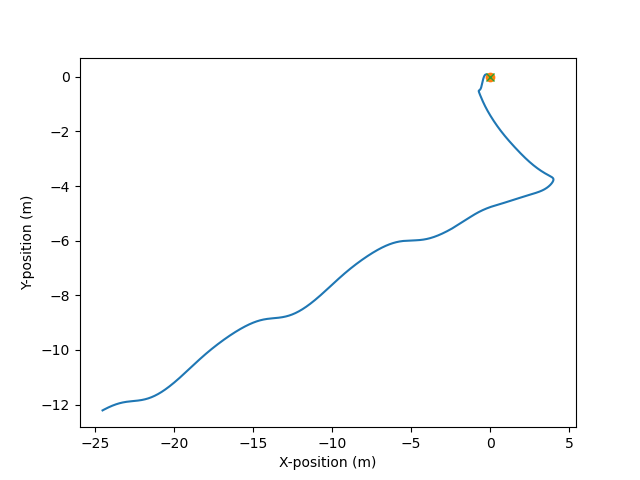
\includegraphics{scenario1/rov-50m/1.0m/usv_position_controlled}
        \caption{1m}
        \label{}
    \end{subfigure}
    \hfill
    \begin{subfigure}[b]{0.48\textwidth}
        \centering
        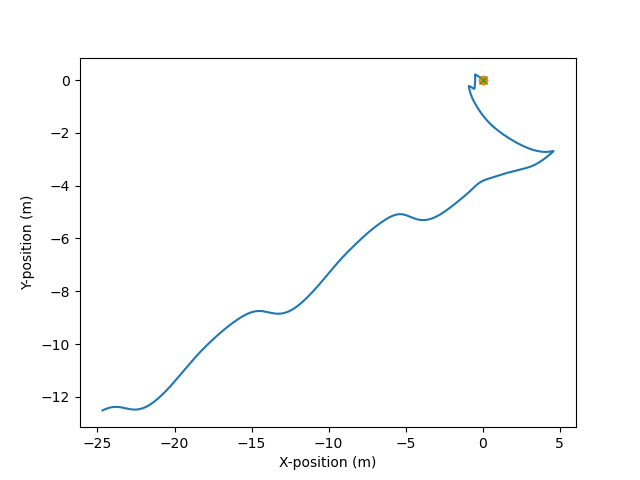
\includegraphics{scenario1/rov-50m/1.5m/usv_position_controlled}
        \caption{1.5m}
        \label{}
    \end{subfigure}
    \vfill
    \begin{subfigure}[b]{0.48\textwidth}
        \centering
        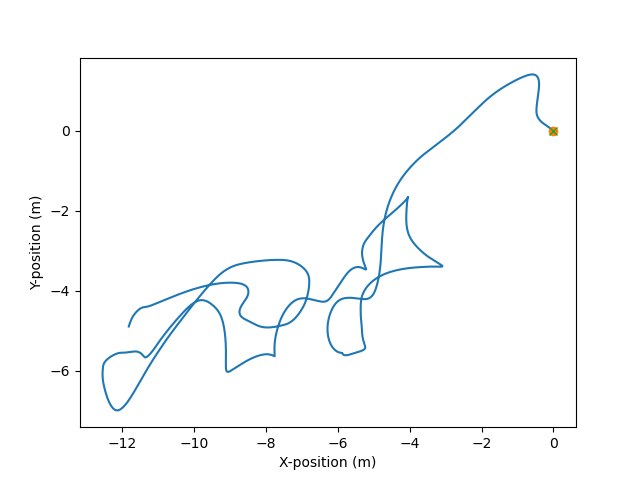
\includegraphics{scenario1/rov-50m/2.0m/usv_position_controlled}
        \caption{2m}
        \label{}
    \end{subfigure}

    \caption{USV position with control at different wave heights, ROV at 50m}
\end{figure}

\begin{figure}
    \centering
    \begin{subfigure}[b]{0.48\textwidth}
        \centering
        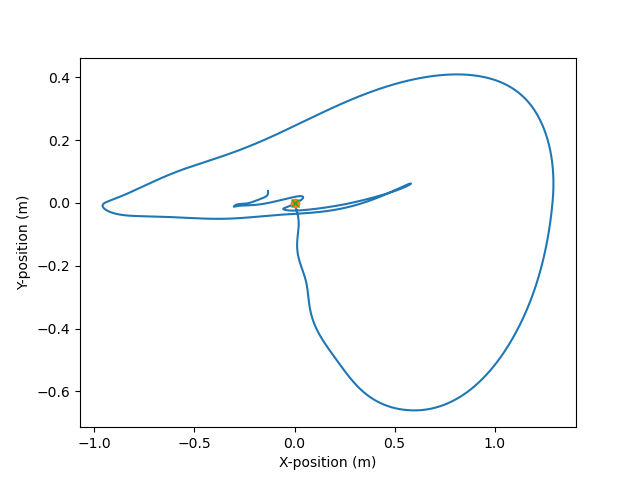
\includegraphics{scenario1/rov-100m/0.0m/usv_position_controlled}
        \caption{0m}
        \label{}
    \end{subfigure}
    \hfill
    \begin{subfigure}[b]{0.48\textwidth}
        \centering
        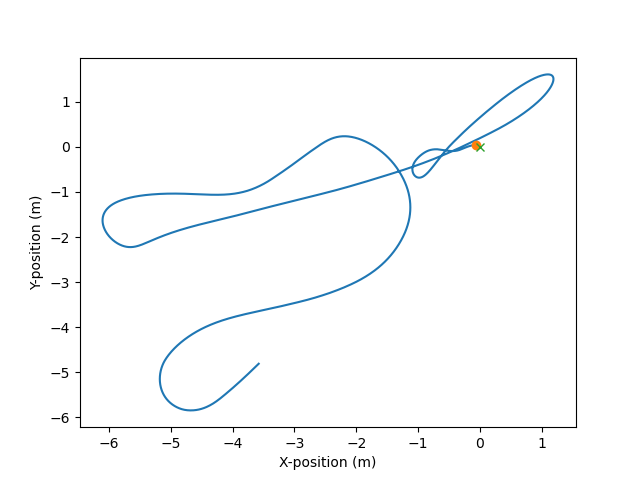
\includegraphics{scenario1/rov-100m/0.5m/usv_position_controlled}
        \caption{0.5m}
        \label{}
    \end{subfigure}
    \vfill
    \begin{subfigure}[b]{0.48\textwidth}
        \centering
        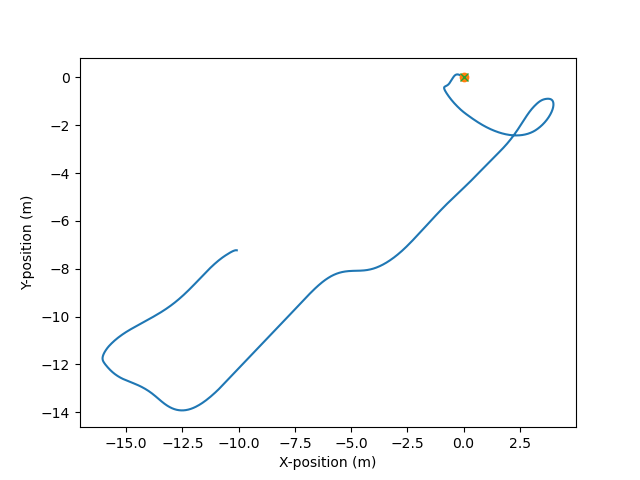
\includegraphics{scenario1/rov-100m/1.0m/usv_position_controlled}
        \caption{1m}
        \label{}
    \end{subfigure}
    \hfill
    \begin{subfigure}[b]{0.48\textwidth}
        \centering
        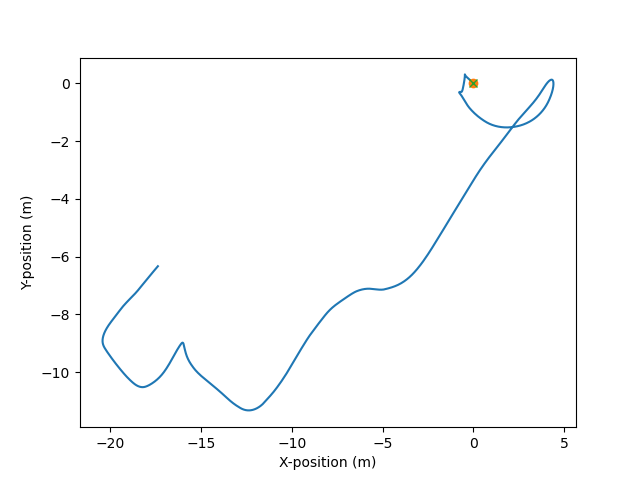
\includegraphics{scenario1/rov-100m/1.5m/usv_position_controlled}
        \caption{1.5m}
        \label{}
    \end{subfigure}
    \vfill
    \begin{subfigure}[b]{0.48\textwidth}
        \centering
        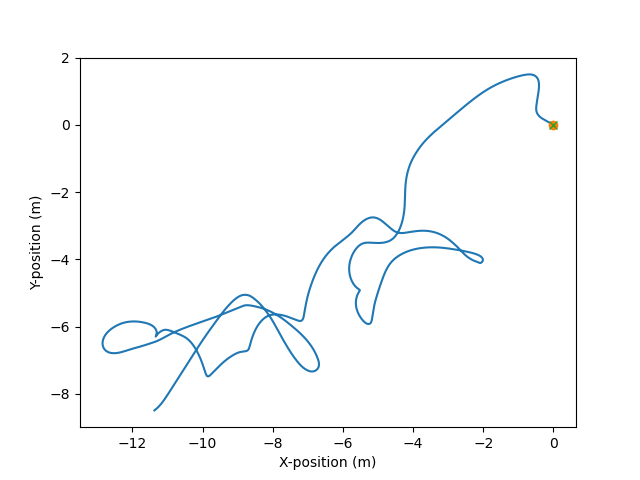
\includegraphics{scenario1/rov-100m/2.0m/usv_position_controlled}
        \caption{2m}
        \label{}
    \end{subfigure}

    \caption{USV position with control at different wave heights, ROV at 100m}
\end{figure}
\FloatBarrier
\section{USV position errors over time}
For the following figures the X- and Y- components of the movement of the USV are shown as blue and yellow respectively.
\subsection{Uncontrolled}
\begin{figure}
    \centering
    \begin{subfigure}[b]{0.48\textwidth}
        \centering
        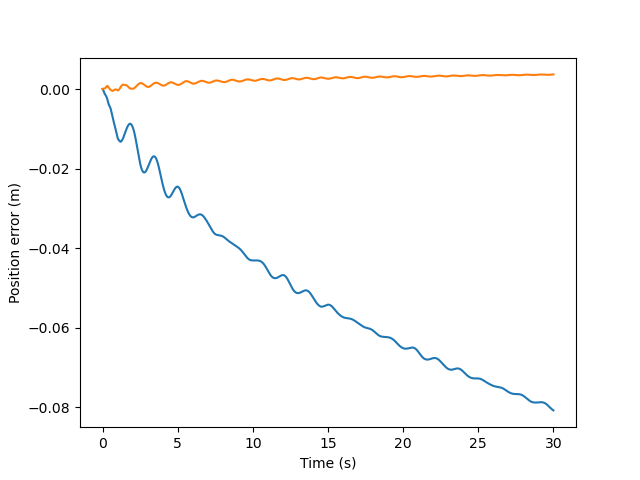
\includegraphics{scenario1/rov-0m/0.0m/usv_pos_error_uncontrolled}
        \caption{0m}
        \label{}
    \end{subfigure}
    \hfill
        \begin{subfigure}[b]{0.48\textwidth}
        \centering
        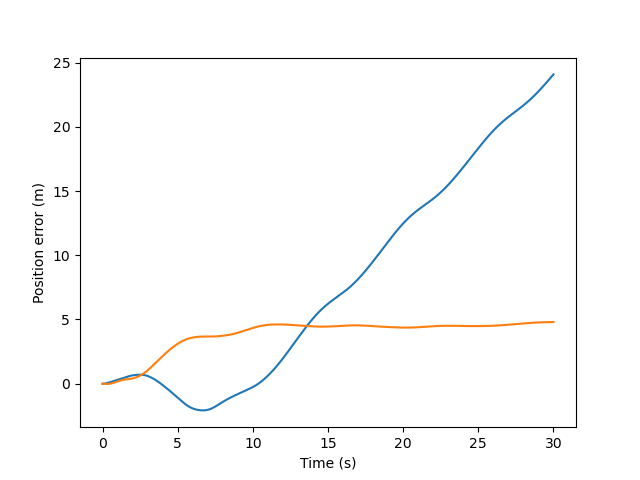
\includegraphics{scenario1/rov-0m/0.5m/usv_pos_error_uncontrolled}
        \caption{0.5m}
        \label{}
    \end{subfigure}
    \vfill
        \begin{subfigure}[b]{0.48\textwidth}
        \centering
        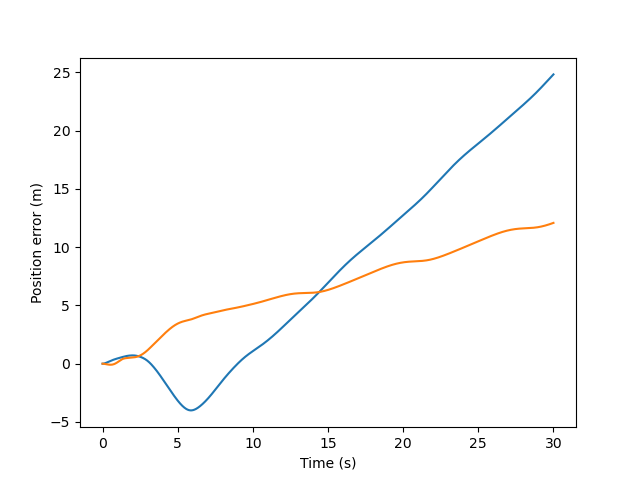
\includegraphics{scenario1/rov-0m/1.0m/usv_pos_error_uncontrolled}
        \caption{1m}
        \label{}
    \end{subfigure}
    \hfill
        \begin{subfigure}[b]{0.48\textwidth}
        \centering
        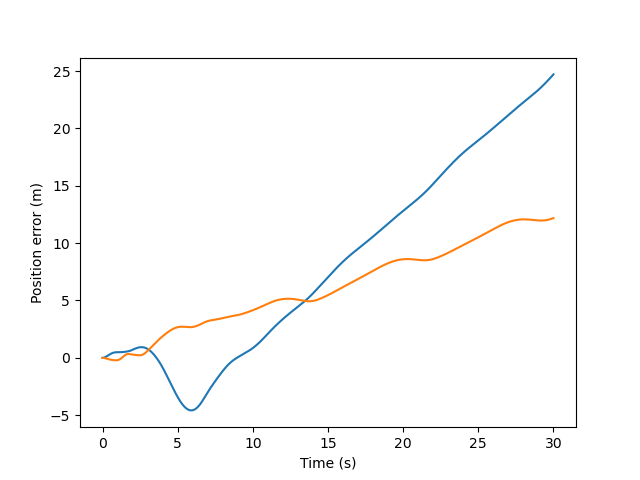
\includegraphics{scenario1/rov-0m/1.5m/usv_pos_error_uncontrolled}
        \caption{1.5m}
        \label{}
    \end{subfigure}
    \vfill
        \begin{subfigure}[b]{0.48\textwidth}
        \centering
        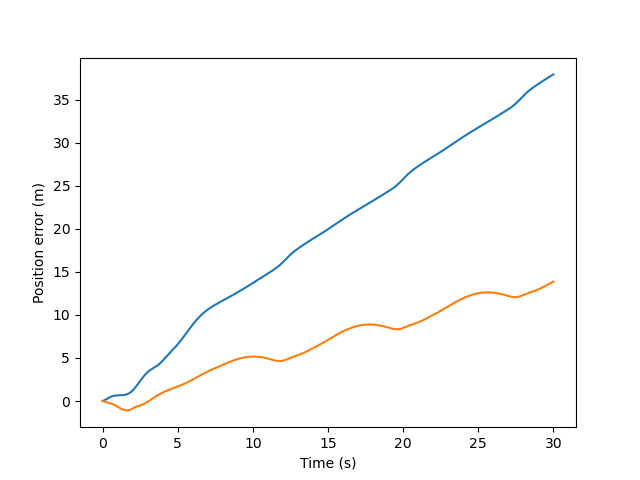
\includegraphics{scenario1/rov-0m/2.0m/usv_pos_error_uncontrolled}
        \caption{2m}
        \label{}
    \end{subfigure}
    \caption{USV position error without control at different wave heights, X-direction as blue, Y-direction as yellow. ROV at 0m}
    \label{}
\end{figure}

\begin{figure}
    \centering
    \begin{subfigure}[b]{0.48\textwidth}
        \centering
        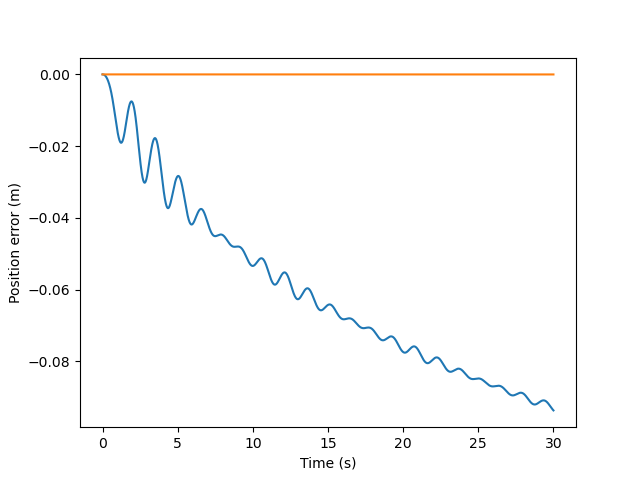
\includegraphics{scenario1/rov-50m/0.0m/usv_pos_error_uncontrolled}
        \caption{0m}
        \label{}
    \end{subfigure}
    \hfill
        \begin{subfigure}[b]{0.48\textwidth}
        \centering
        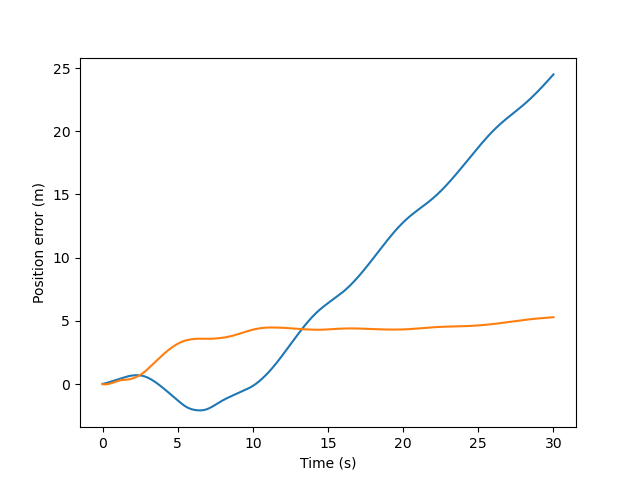
\includegraphics{scenario1/rov-50m/0.5m/usv_pos_error_uncontrolled}
        \caption{0.5m}
        \label{}
    \end{subfigure}
    \vfill
        \begin{subfigure}[b]{0.48\textwidth}
        \centering
        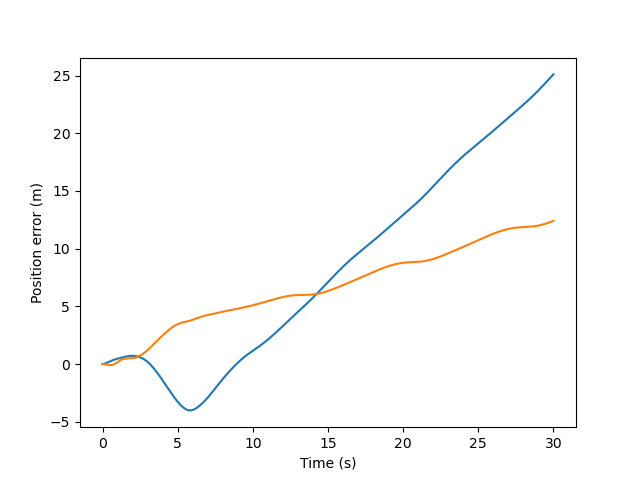
\includegraphics{scenario1/rov-50m/1.0m/usv_pos_error_uncontrolled}
        \caption{1m}
        \label{}
    \end{subfigure}
    \hfill
        \begin{subfigure}[b]{0.48\textwidth}
        \centering
        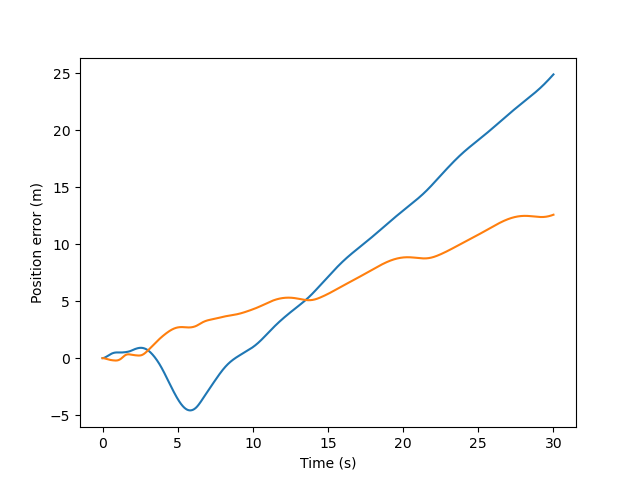
\includegraphics{scenario1/rov-50m/1.5m/usv_pos_error_uncontrolled}
        \caption{1.5m}
        \label{}
    \end{subfigure}
    \vfill
        \begin{subfigure}[b]{0.48\textwidth}
        \centering
        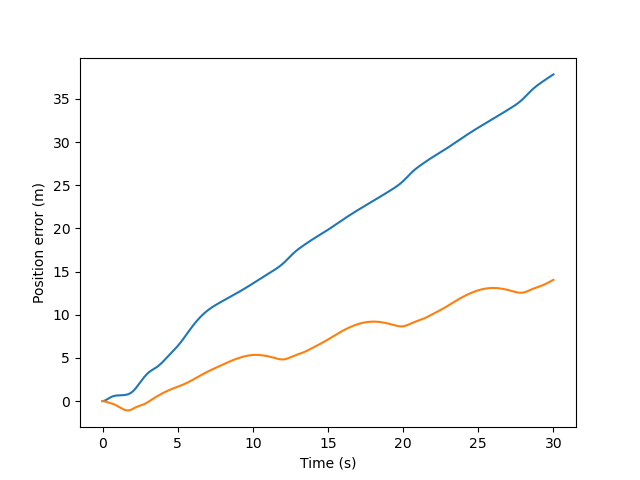
\includegraphics{scenario1/rov-50m/2.0m/usv_pos_error_uncontrolled}
        \caption{2m}
        \label{}
    \end{subfigure}
    \caption{USV position error without control at different wave heights, X-direction as blue, Y-direction as yellow. ROV at 50m}
    \label{}
\end{figure}

\begin{figure}
    \centering
    \begin{subfigure}[b]{0.48\textwidth}
        \centering
        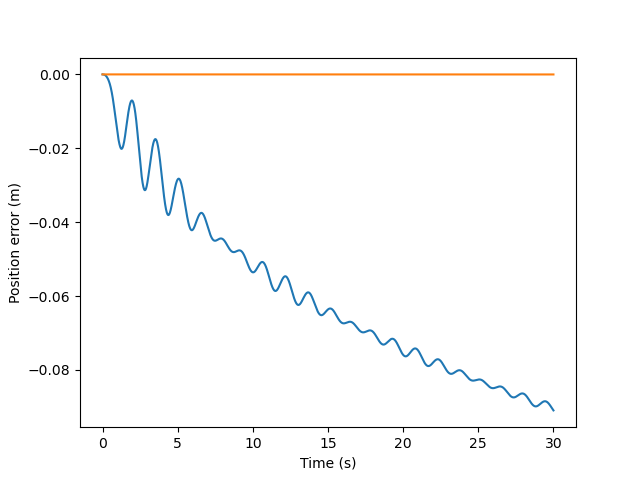
\includegraphics{scenario1/rov-100m/0.0m/usv_pos_error_uncontrolled}
        \caption{0m}
        \label{}
    \end{subfigure}
    \hfill
        \begin{subfigure}[b]{0.48\textwidth}
        \centering
        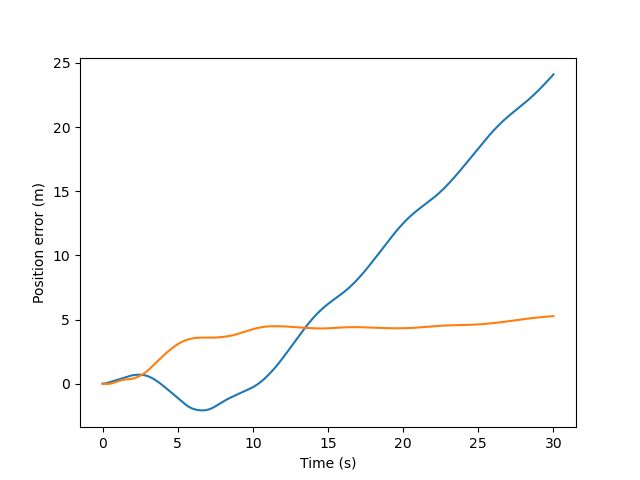
\includegraphics{scenario1/rov-100m/0.5m/usv_pos_error_uncontrolled}
        \caption{0.5m}
        \label{}
    \end{subfigure}
    \vfill
        \begin{subfigure}[b]{0.48\textwidth}
        \centering
        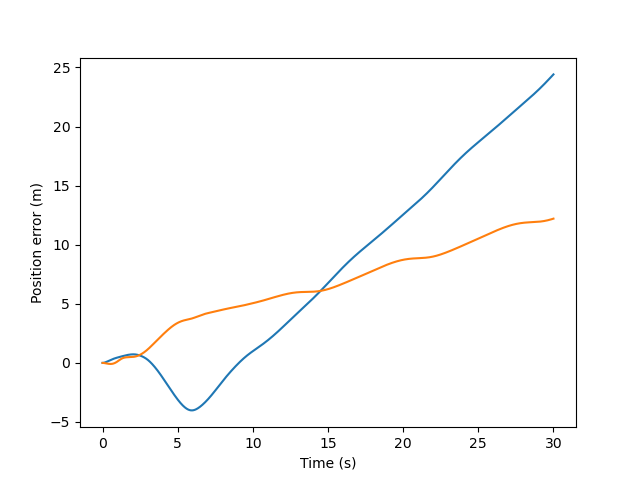
\includegraphics{scenario1/rov-100m/1.0m/usv_pos_error_uncontrolled}
        \caption{1m}
        \label{}
    \end{subfigure}
    \hfill
        \begin{subfigure}[b]{0.48\textwidth}
        \centering
        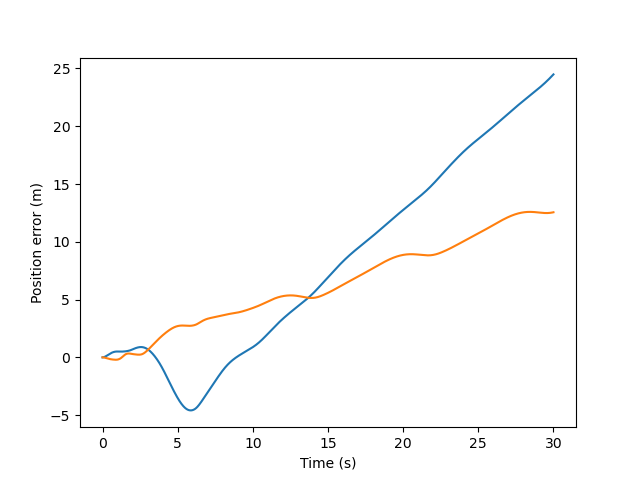
\includegraphics{scenario1/rov-100m/1.5m/usv_pos_error_uncontrolled}
        \caption{1.5m}
        \label{}
    \end{subfigure}
    \vfill
        \begin{subfigure}[b]{0.48\textwidth}
        \centering
        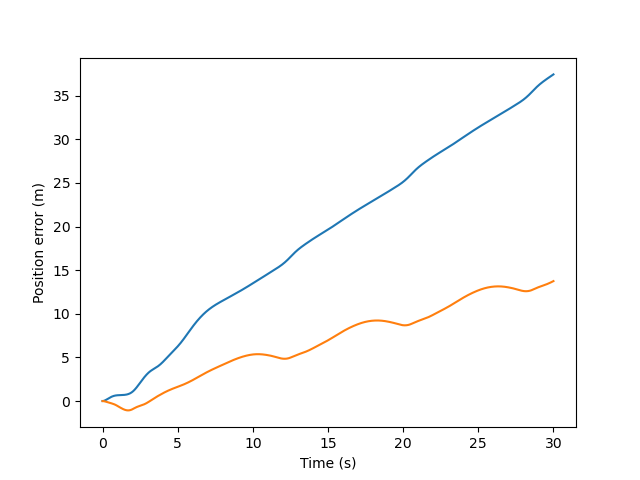
\includegraphics{scenario1/rov-100m/2.0m/usv_pos_error_uncontrolled}
        \caption{2m}
        \label{}
    \end{subfigure}
    \caption{USV position error without control at different wave heights, X-direction as blue, Y-direction as yellow. ROV at 100m}
    \label{}
\end{figure}
\FloatBarrier
\subsection{Controlled}
\begin{figure}
    \centering
    \begin{subfigure}[b]{0.48\textwidth}
        \centering
        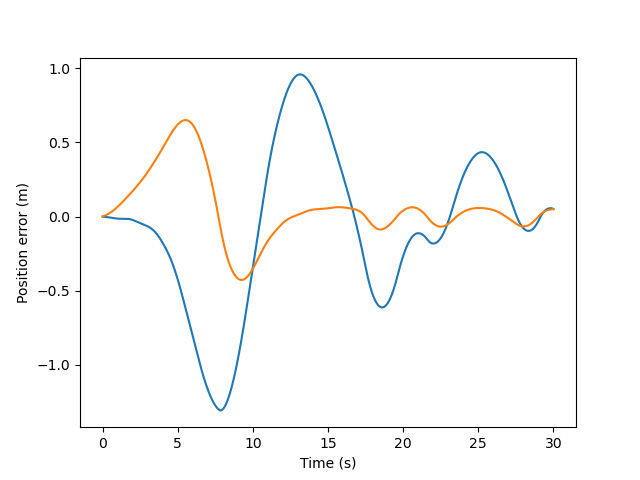
\includegraphics{scenario1/rov-0m/0.0m/usv_pos_error_controlled}
        \caption{0m}
        \label{}
    \end{subfigure}
    \hfill
        \begin{subfigure}[b]{0.48\textwidth}
        \centering
        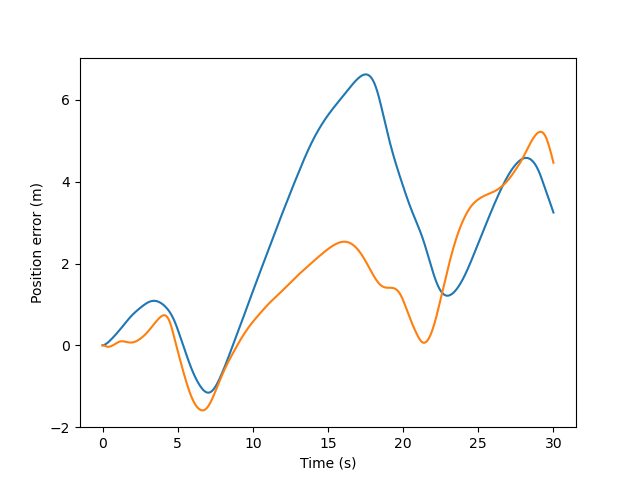
\includegraphics{scenario1/rov-0m/0.5m/usv_pos_error_controlled}
        \caption{0.5m}
        \label{}
    \end{subfigure}
    \vfill
        \begin{subfigure}[b]{0.48\textwidth}
        \centering
        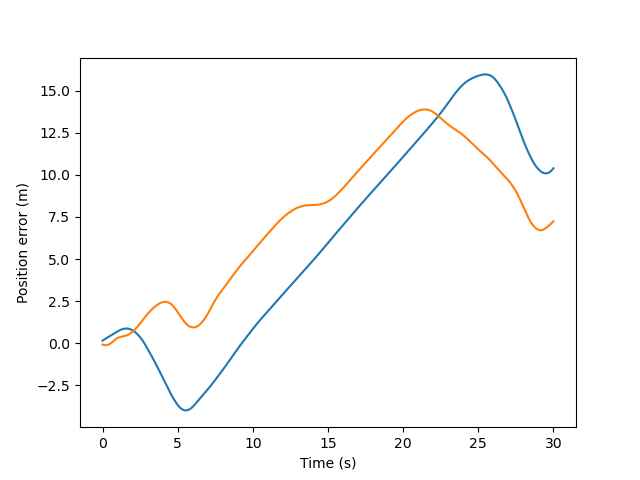
\includegraphics{scenario1/rov-0m/1.0m/usv_pos_error_controlled}
        \caption{1m}
        \label{}
    \end{subfigure}
    \hfill
        \begin{subfigure}[b]{0.48\textwidth}
        \centering
        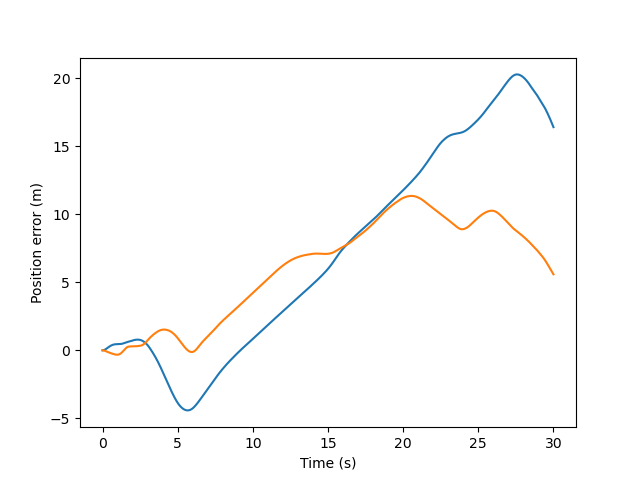
\includegraphics{scenario1/rov-0m/1.5m/usv_pos_error_controlled}
        \caption{1.5m}
        \label{}
    \end{subfigure}
    \vfill
        \begin{subfigure}[b]{0.48\textwidth}
        \centering
        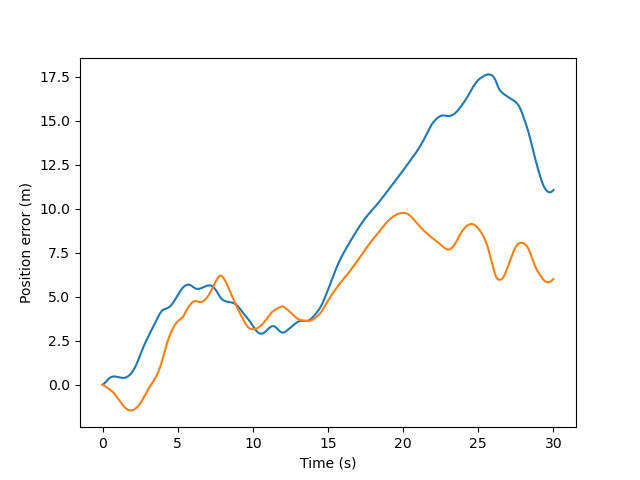
\includegraphics{scenario1/rov-0m/2.0m/usv_pos_error_controlled}
        \caption{2m}
        \label{}
    \end{subfigure}
    \caption{USV position error with control at different wave heights, X-direction as blue, Y-direction as yellow. ROV at 0m}
    \label{}
\end{figure}

\begin{figure}
    \centering
    \begin{subfigure}[b]{0.48\textwidth}
        \centering
        \includegraphics{scenario1/rov-50m/0.0m/usv_pos_error_controlled}
        \caption{0m}
        \label{}
    \end{subfigure}
    \hfill
        \begin{subfigure}[b]{0.48\textwidth}
        \centering
        \includegraphics{scenario1/rov-50m/0.5m/usv_pos_error_controlled}
        \caption{0.5m}
        \label{}
    \end{subfigure}
    \vfill
        \begin{subfigure}[b]{0.48\textwidth}
        \centering
        \includegraphics{scenario1/rov-50m/1.0m/usv_pos_error_controlled}
        \caption{1m}
        \label{}
    \end{subfigure}
    \hfill
        \begin{subfigure}[b]{0.48\textwidth}
        \centering
        \includegraphics{scenario1/rov-50m/1.5m/usv_pos_error_controlled}
        \caption{1.5m}
        \label{}
    \end{subfigure}
    \vfill
        \begin{subfigure}[b]{0.48\textwidth}
        \centering
        \includegraphics{scenario1/rov-50m/2.0m/usv_pos_error_controlled}
        \caption{2m}
        \label{}
    \end{subfigure}
    \caption{USV position error with control at different wave heights, X-direction as blue, Y-direction as yellow. ROV at 50m}
    \label{}
\end{figure}

\begin{figure}
    \centering
    \begin{subfigure}[b]{0.48\textwidth}
        \centering
        \includegraphics{scenario1/rov-100m/0.0m/usv_pos_error_controlled}
        \caption{0m}
        \label{}
    \end{subfigure}
    \hfill
        \begin{subfigure}[b]{0.48\textwidth}
        \centering
        \includegraphics{scenario1/rov-100m/0.5m/usv_pos_error_controlled}
        \caption{0.5m}
        \label{}
    \end{subfigure}
    \vfill
        \begin{subfigure}[b]{0.48\textwidth}
        \centering
        \includegraphics{scenario1/rov-100m/1.0m/usv_pos_error_controlled}
        \caption{1m}
        \label{}
    \end{subfigure}
    \hfill
        \begin{subfigure}[b]{0.48\textwidth}
        \centering
        \includegraphics{scenario1/rov-100m/1.5m/usv_pos_error_controlled}
        \caption{1.5m}
        \label{}
    \end{subfigure}
    \vfill
        \begin{subfigure}[b]{0.48\textwidth}
        \centering
        \includegraphics{scenario1/rov-100m/2.0m/usv_pos_error_controlled}
        \caption{2m}
        \label{}
    \end{subfigure}
    \caption{USV position error with control at different wave heights, X-direction as blue, Y-direction as yellow. ROV at 100m}
    \label{}
\end{figure}
\FloatBarrier
\section{USV heading error}
\subsection{Uncontrolled}
\begin{figure}
    \centering
    \begin{subfigure}[b]{0.48\textwidth}
        \centering
        \includegraphics{scenario1/rov-0m/0.0m/usv_heading_error_uncontrolled}
        \caption{0m}
        \label{}
    \end{subfigure}
    \hfill
    \begin{subfigure}[b]{0.48\textwidth}
        \centering
        \includegraphics{scenario1/rov-0m/0.5m/usv_heading_error_uncontrolled}
        \caption{0.5m}
        \label{}
    \end{subfigure}
    \vfill
    \begin{subfigure}[b]{0.48\textwidth}
        \centering
        \includegraphics{scenario1/rov-0m/1.0m/usv_heading_error_uncontrolled}
        \caption{1m}
        \label{}
    \end{subfigure}
    \hfill
    \begin{subfigure}[b]{0.48\textwidth}
        \centering
        \includegraphics{scenario1/rov-0m/1.5m/usv_heading_error_uncontrolled}
        \caption{1.5m}
        \label{}
    \end{subfigure}
    \vfill
    \begin{subfigure}[b]{0.48\textwidth}
        \centering
        \includegraphics{scenario1/rov-0m/2.0m/usv_heading_error_uncontrolled}
        \caption{2m}
        \label{}
    \end{subfigure}

    \caption{USV heading error at different wave heights, ROV at 0m, without control}
\end{figure}

\begin{figure}
    \centering
    \begin{subfigure}[b]{0.48\textwidth}
        \centering
        \includegraphics{scenario1/rov-50m/0.0m/usv_heading_error_uncontrolled}
        \caption{0m}
        \label{}
    \end{subfigure}
    \hfill
    \begin{subfigure}[b]{0.48\textwidth}
        \centering
        \includegraphics{scenario1/rov-50m/0.5m/usv_heading_error_uncontrolled}
        \caption{0.5m}
        \label{}
    \end{subfigure}
    \vfill
    \begin{subfigure}[b]{0.48\textwidth}
        \centering
        \includegraphics{scenario1/rov-50m/1.0m/usv_heading_error_uncontrolled}
        \caption{1m}
        \label{}
    \end{subfigure}
    \hfill
    \begin{subfigure}[b]{0.48\textwidth}
        \centering
        \includegraphics{scenario1/rov-50m/1.5m/usv_heading_error_uncontrolled}
        \caption{1.5m}
        \label{}
    \end{subfigure}
    \vfill
    \begin{subfigure}[b]{0.48\textwidth}
        \centering
        \includegraphics{scenario1/rov-50m/2.0m/usv_heading_error_uncontrolled}
        \caption{2m}
        \label{}
    \end{subfigure}

    \caption{USV heading error at different wave heights, ROV at 50m, without control}
\end{figure}

\begin{figure}
    \centering
    \begin{subfigure}[b]{0.48\textwidth}
        \centering
        \includegraphics{scenario1/rov-100m/0.0m/usv_heading_error_uncontrolled}
        \caption{0m}
        \label{}
    \end{subfigure}
    \hfill
    \begin{subfigure}[b]{0.48\textwidth}
        \centering
        \includegraphics{scenario1/rov-100m/0.5m/usv_heading_error_uncontrolled}
        \caption{0.5m}
        \label{}
    \end{subfigure}
    \vfill
    \begin{subfigure}[b]{0.48\textwidth}
        \centering
        \includegraphics{scenario1/rov-100m/1.0m/usv_heading_error_uncontrolled}
        \caption{1m}
        \label{}
    \end{subfigure}
    \hfill
    \begin{subfigure}[b]{0.48\textwidth}
        \centering
        \includegraphics{scenario1/rov-100m/1.5m/usv_heading_error_uncontrolled}
        \caption{1.5m}
        \label{}
    \end{subfigure}
    \vfill
    \begin{subfigure}[b]{0.48\textwidth}
        \centering
        \includegraphics{scenario1/rov-100m/2.0m/usv_heading_error_uncontrolled}
        \caption{2m}
        \label{}
    \end{subfigure}

    \caption{USV heading error at different wave heights, ROV at 100m, without control}
\end{figure}
\FloatBarrier
\subsection{Controlled}
\begin{figure}
    \centering
    \begin{subfigure}[b]{0.48\textwidth}
        \centering
        \includegraphics{scenario1/rov-0m/0.0m/usv_heading_error_controlled}
        \caption{0m}
        \label{}
    \end{subfigure}
    \hfill
    \begin{subfigure}[b]{0.48\textwidth}
        \centering
        \includegraphics{scenario1/rov-0m/0.5m/usv_heading_error_controlled}
        \caption{0.5m}
        \label{}
    \end{subfigure}
    \vfill
    \begin{subfigure}[b]{0.48\textwidth}
        \centering
        \includegraphics{scenario1/rov-0m/1.0m/usv_heading_error_controlled}
        \caption{1m}
        \label{}
    \end{subfigure}
    \hfill
    \begin{subfigure}[b]{0.48\textwidth}
        \centering
        \includegraphics{scenario1/rov-0m/1.5m/usv_heading_error_controlled}
        \caption{1.5m}
        \label{}
    \end{subfigure}
    \vfill
    \begin{subfigure}[b]{0.48\textwidth}
        \centering
        \includegraphics{scenario1/rov-0m/2.0m/usv_heading_error_controlled}
        \caption{2m}
        \label{}
    \end{subfigure}

    \caption{USV heading error at different wave heights, ROV at 0m, with control}
\end{figure}

\begin{figure}
    \centering
    \begin{subfigure}[b]{0.48\textwidth}
        \centering
        \includegraphics{scenario1/rov-50m/0.0m/usv_heading_error_controlled}
        \caption{0m}
        \label{}
    \end{subfigure}
    \hfill
    \begin{subfigure}[b]{0.48\textwidth}
        \centering
        \includegraphics{scenario1/rov-50m/0.5m/usv_heading_error_controlled}
        \caption{0.5m}
        \label{}
    \end{subfigure}
    \vfill
    \begin{subfigure}[b]{0.48\textwidth}
        \centering
        \includegraphics{scenario1/rov-50m/1.0m/usv_heading_error_controlled}
        \caption{1m}
        \label{}
    \end{subfigure}
    \hfill
    \begin{subfigure}[b]{0.48\textwidth}
        \centering
        \includegraphics{scenario1/rov-50m/1.5m/usv_heading_error_controlled}
        \caption{1.5m}
        \label{}
    \end{subfigure}
    \vfill
    \begin{subfigure}[b]{0.48\textwidth}
        \centering
        \includegraphics{scenario1/rov-50m/2.0m/usv_heading_error_controlled}
        \caption{2m}
        \label{}
    \end{subfigure}

    \caption{USV heading error at different wave heights, ROV at 50m, with control}
\end{figure}

\begin{figure}
    \centering
    \begin{subfigure}[b]{0.48\textwidth}
        \centering
        \includegraphics{scenario1/rov-100m/0.0m/usv_heading_error_controlled}
        \caption{0m}
        \label{}
    \end{subfigure}
    \hfill
    \begin{subfigure}[b]{0.48\textwidth}
        \centering
        \includegraphics{scenario1/rov-100m/0.5m/usv_heading_error_controlled}
        \caption{0.5m}
        \label{}
    \end{subfigure}
    \vfill
    \begin{subfigure}[b]{0.48\textwidth}
        \centering
        \includegraphics{scenario1/rov-100m/1.0m/usv_heading_error_controlled}
        \caption{1m}
        \label{}
    \end{subfigure}
    \hfill
    \begin{subfigure}[b]{0.48\textwidth}
        \centering
        \includegraphics{scenario1/rov-100m/1.5m/usv_heading_error_controlled}
        \caption{1.5m}
        \label{}
    \end{subfigure}
    \vfill
    \begin{subfigure}[b]{0.48\textwidth}
        \centering
        \includegraphics{scenario1/rov-100m/2.0m/usv_heading_error_controlled}
        \caption{2m}
        \label{}
    \end{subfigure}

    \caption{USV heading error at different wave heights, ROV at 100m, with control}
\end{figure}
\FloatBarrier
\section{USV applied forces}
\subsection{Lateral forces}
\begin{figure}
    \centering
    \begin{subfigure}[b]{0.48\textwidth}
        \centering
        \includegraphics{scenario1/rov-0m/0.0m/usv_forces}
        \caption{0m}
        \label{}
    \end{subfigure}
    \hfill
    \begin{subfigure}[b]{0.48\textwidth}
        \centering
        \includegraphics{scenario1/rov-0m/0.5m/usv_forces}
        \caption{0.5m}
        \label{}
    \end{subfigure}
    \vfill
    \begin{subfigure}[b]{0.48\textwidth}
        \centering
        \includegraphics{scenario1/rov-0m/1.0m/usv_forces}
        \caption{1m}
        \label{}
    \end{subfigure}
    \hfill
    \begin{subfigure}[b]{0.48\textwidth}
        \centering
        \includegraphics{scenario1/rov-0m/1.5m/usv_forces}
        \caption{1.5m}
        \label{}
    \end{subfigure}
    \vfill
    \begin{subfigure}[b]{0.48\textwidth}
        \centering
        \includegraphics{scenario1/rov-0m/2.0m/usv_forces}
        \caption{2m}
        \label{}
    \end{subfigure}

    \caption{USV lateral forces applied by controller at different wave heights, ROV at 0m}
\end{figure}
\begin{figure}
    \centering
    \begin{subfigure}[b]{0.48\textwidth}
        \centering
        \includegraphics{scenario1/rov-50m/0.0m/usv_forces}
        \caption{0m}
        \label{}
    \end{subfigure}
    \hfill
    \begin{subfigure}[b]{0.48\textwidth}
        \centering
        \includegraphics{scenario1/rov-50m/0.5m/usv_forces}
        \caption{0.5m}
        \label{}
    \end{subfigure}
    \vfill
    \begin{subfigure}[b]{0.48\textwidth}
        \centering
        \includegraphics{scenario1/rov-50m/1.0m/usv_forces}
        \caption{1m}
        \label{}
    \end{subfigure}
    \hfill
    \begin{subfigure}[b]{0.48\textwidth}
        \centering
        \includegraphics{scenario1/rov-50m/1.5m/usv_forces}
        \caption{1.5m}
        \label{}
    \end{subfigure}
    \vfill
    \begin{subfigure}[b]{0.48\textwidth}
        \centering
        \includegraphics{scenario1/rov-50m/2.0m/usv_forces}
        \caption{2m}
        \label{}
    \end{subfigure}

    \caption{USV lateral forces applied by controller at different wave heights, ROV at 50m}
\end{figure}
\begin{figure}
    \centering
    \begin{subfigure}[b]{0.48\textwidth}
        \centering
        \includegraphics{scenario1/rov-100m/0.0m/usv_forces}
        \caption{0m}
        \label{}
    \end{subfigure}
    \hfill
    \begin{subfigure}[b]{0.48\textwidth}
        \centering
        \includegraphics{scenario1/rov-100m/0.5m/usv_forces}
        \caption{0.5m}
        \label{}
    \end{subfigure}
    \vfill
    \begin{subfigure}[b]{0.48\textwidth}
        \centering
        \includegraphics{scenario1/rov-100m/1.0m/usv_forces}
        \caption{1m}
        \label{}
    \end{subfigure}
    \hfill
    \begin{subfigure}[b]{0.48\textwidth}
        \centering
        \includegraphics{scenario1/rov-100m/1.5m/usv_forces}
        \caption{1.5m}
        \label{}
    \end{subfigure}
    \vfill
    \begin{subfigure}[b]{0.48\textwidth}
        \centering
        \includegraphics{scenario1/rov-100m/2.0m/usv_forces}
        \caption{2m}
        \label{}
    \end{subfigure}

    \caption{USV lateral forces applied by controller at different wave heights, ROV at 100m}
\end{figure}
\FloatBarrier
\subsection{Torque}
\begin{figure}
    \centering
    \begin{subfigure}[b]{0.48\textwidth}
        \centering
        \includegraphics{scenario1/rov-0m/0.0m/usv_torque}
        \caption{0m}
        \label{}
    \end{subfigure}
    \hfill
    \begin{subfigure}[b]{0.48\textwidth}
        \centering
        \includegraphics{scenario1/rov-0m/0.5m/usv_torque}
        \caption{0.5m}
        \label{}
    \end{subfigure}
    \vfill
    \begin{subfigure}[b]{0.48\textwidth}
        \centering
        \includegraphics{scenario1/rov-0m/1.0m/usv_torque}
        \caption{1m}
        \label{}
    \end{subfigure}
    \hfill
    \begin{subfigure}[b]{0.48\textwidth}
        \centering
        \includegraphics{scenario1/rov-0m/1.5m/usv_torque}
        \caption{1.5m}
        \label{}
    \end{subfigure}
    \vfill
    \begin{subfigure}[b]{0.48\textwidth}
        \centering
        \includegraphics{scenario1/rov-0m/2.0m/usv_torque}
        \caption{2m}
        \label{}
    \end{subfigure}

    \caption{USV torque applied by controller at different wave heights, ROV at 0m}
\end{figure}
\begin{figure}
    \centering
    \begin{subfigure}[b]{0.48\textwidth}
        \centering
        \includegraphics{scenario1/rov-50m/0.0m/usv_torque}
        \caption{0m}
        \label{}
    \end{subfigure}
    \hfill
    \begin{subfigure}[b]{0.48\textwidth}
        \centering
        \includegraphics{scenario1/rov-50m/0.5m/usv_torque}
        \caption{0.5m}
        \label{}
    \end{subfigure}
    \vfill
    \begin{subfigure}[b]{0.48\textwidth}
        \centering
        \includegraphics{scenario1/rov-50m/1.0m/usv_torque}
        \caption{1m}
        \label{}
    \end{subfigure}
    \hfill
    \begin{subfigure}[b]{0.48\textwidth}
        \centering
        \includegraphics{scenario1/rov-50m/1.5m/usv_torque}
        \caption{1.5m}
        \label{}
    \end{subfigure}
    \vfill
    \begin{subfigure}[b]{0.48\textwidth}
        \centering
        \includegraphics{scenario1/rov-50m/2.0m/usv_torque}
        \caption{2m}
        \label{}
    \end{subfigure}

    \caption{USV torque applied by controller at different wave heights, ROV at 50m}
\end{figure}
\begin{figure}
    \centering
    \begin{subfigure}[b]{0.48\textwidth}
        \centering
        \includegraphics{scenario1/rov-100m/0.0m/usv_torque}
        \caption{0m}
        \label{}
    \end{subfigure}
    \hfill
    \begin{subfigure}[b]{0.48\textwidth}
        \centering
        \includegraphics{scenario1/rov-100m/0.5m/usv_torque}
        \caption{0.5m}
        \label{}
    \end{subfigure}
    \vfill
    \begin{subfigure}[b]{0.48\textwidth}
        \centering
        \includegraphics{scenario1/rov-100m/1.0m/usv_torque}
        \caption{1m}
        \label{}
    \end{subfigure}
    \hfill
    \begin{subfigure}[b]{0.48\textwidth}
        \centering
        \includegraphics{scenario1/rov-100m/1.5m/usv_torque}
        \caption{1.5m}
        \label{}
    \end{subfigure}
    \vfill
    \begin{subfigure}[b]{0.48\textwidth}
        \centering
        \includegraphics{scenario1/rov-100m/2.0m/usv_torque}
        \caption{2m}
        \label{}
    \end{subfigure}

    \caption{USV torque applied by controller at different wave heights, ROV at 100m}
\end{figure}

\FloatBarrier
\section{ROV position error over time}
\subsection{Uncontrolled}
\begin{figure}
    \centering
    \begin{subfigure}[b]{0.48\textwidth}
        \centering
        \includegraphics{scenario1/rov-0m/0.0m/rov_position_error_uncontrolled}
        \caption{0m}
        \label{}
    \end{subfigure}
    \hfill
    \begin{subfigure}[b]{0.48\textwidth}
        \centering
        \includegraphics{scenario1/rov-0m/0.5m/rov_position_error_uncontrolled}
        \caption{0.5m}
        \label{}
    \end{subfigure}
    \vfill
    \begin{subfigure}[b]{0.48\textwidth}
        \centering
        \includegraphics{scenario1/rov-0m/1.0m/rov_position_error_uncontrolled}
        \caption{1m}
        \label{}
    \end{subfigure}
    \hfill
    \begin{subfigure}[b]{0.48\textwidth}
        \centering
        \includegraphics{scenario1/rov-0m/1.5m/rov_position_error_uncontrolled}
        \caption{1.5m}
        \label{}
    \end{subfigure}
    \vfill
    \begin{subfigure}[b]{0.48\textwidth}
        \centering
        \includegraphics{scenario1/rov-0m/2.0m/rov_position_error_uncontrolled}
        \caption{2m}
        \label{}
    \end{subfigure}

    \caption{ROV position error without control at different wave heights, ROV at 0m}
\end{figure}

\begin{figure}
    \centering
    \begin{subfigure}[b]{0.48\textwidth}
        \centering
        \includegraphics{scenario1/rov-50m/0.0m/rov_position_error_uncontrolled}
        \caption{0m}
        \label{}
    \end{subfigure}
    \hfill
    \begin{subfigure}[b]{0.48\textwidth}
        \centering
        \includegraphics{scenario1/rov-50m/0.5m/rov_position_error_uncontrolled}
        \caption{0.5m}
        \label{}
    \end{subfigure}
    \vfill
    \begin{subfigure}[b]{0.48\textwidth}
        \centering
        \includegraphics{scenario1/rov-50m/1.0m/rov_position_error_uncontrolled}
        \caption{1m}
        \label{}
    \end{subfigure}
    \hfill
    \begin{subfigure}[b]{0.48\textwidth}
        \centering
        \includegraphics{scenario1/rov-50m/1.5m/rov_position_error_uncontrolled}
        \caption{1.5m}
        \label{}
    \end{subfigure}
    \vfill
    \begin{subfigure}[b]{0.48\textwidth}
        \centering
        \includegraphics{scenario1/rov-50m/2.0m/rov_position_error_uncontrolled}
        \caption{2m}
        \label{}
    \end{subfigure}

    \caption{ROV position error without control at different wave heights, ROV at 50m}
\end{figure}

\begin{figure}
    \centering
    \begin{subfigure}[b]{0.48\textwidth}
        \centering
        \includegraphics{scenario1/rov-100m/0.0m/rov_position_error_uncontrolled}
        \caption{0m}
        \label{}
    \end{subfigure}
    \hfill
    \begin{subfigure}[b]{0.48\textwidth}
        \centering
        \includegraphics{scenario1/rov-100m/0.5m/rov_position_error_uncontrolled}
        \caption{0.5m}
        \label{}
    \end{subfigure}
    \vfill
    \begin{subfigure}[b]{0.48\textwidth}
        \centering
        \includegraphics{scenario1/rov-100m/1.0m/rov_position_error_uncontrolled}
        \caption{1m}
        \label{}
    \end{subfigure}
    \hfill
    \begin{subfigure}[b]{0.48\textwidth}
        \centering
        \includegraphics{scenario1/rov-100m/1.5m/rov_position_error_uncontrolled}
        \caption{1.5m}
        \label{}
    \end{subfigure}
    \vfill
    \begin{subfigure}[b]{0.48\textwidth}
        \centering
        \includegraphics{scenario1/rov-100m/2.0m/rov_position_error_uncontrolled}
        \caption{2m}
        \label{}
    \end{subfigure}

    \caption{ROV position error without control at different wave heights, ROV at 100m}
\end{figure}
\FloatBarrier
\subsection{Controlled}
\begin{figure}
    \centering
    \begin{subfigure}[b]{0.48\textwidth}
        \centering
        \includegraphics{scenario1/rov-0m/0.0m/rov_position_error_controlled}
        \caption{0m}
        \label{}
    \end{subfigure}
    \hfill
    \begin{subfigure}[b]{0.48\textwidth}
        \centering
        \includegraphics{scenario1/rov-0m/0.5m/rov_position_error_controlled}
        \caption{0.5m}
        \label{}
    \end{subfigure}
    \vfill
    \begin{subfigure}[b]{0.48\textwidth}
        \centering
        \includegraphics{scenario1/rov-0m/1.0m/rov_position_error_controlled}
        \caption{1m}
        \label{}
    \end{subfigure}
    \hfill
    \begin{subfigure}[b]{0.48\textwidth}
        \centering
        \includegraphics{scenario1/rov-0m/1.5m/rov_position_error_controlled}
        \caption{1.5m}
        \label{}
    \end{subfigure}
    \vfill
    \begin{subfigure}[b]{0.48\textwidth}
        \centering
        \includegraphics{scenario1/rov-0m/2.0m/rov_position_error_controlled}
        \caption{2m}
        \label{}
    \end{subfigure}

    \caption{ROV position error with control at different wave heights, ROV at 0m}
\end{figure}

\begin{figure}
    \centering
    \begin{subfigure}[b]{0.48\textwidth}
        \centering
        \includegraphics{scenario1/rov-50m/0.0m/rov_position_error_controlled}
        \caption{0m}
        \label{}
    \end{subfigure}
    \hfill
    \begin{subfigure}[b]{0.48\textwidth}
        \centering
        \includegraphics{scenario1/rov-50m/0.5m/rov_position_error_controlled}
        \caption{0.5m}
        \label{}
    \end{subfigure}
    \vfill
    \begin{subfigure}[b]{0.48\textwidth}
        \centering
        \includegraphics{scenario1/rov-50m/1.0m/rov_position_error_controlled}
        \caption{1m}
        \label{}
    \end{subfigure}
    \hfill
    \begin{subfigure}[b]{0.48\textwidth}
        \centering
        \includegraphics{scenario1/rov-50m/1.5m/rov_position_error_controlled}
        \caption{1.5m}
        \label{}
    \end{subfigure}
    \vfill
    \begin{subfigure}[b]{0.48\textwidth}
        \centering
        \includegraphics{scenario1/rov-50m/2.0m/rov_position_error_controlled}
        \caption{2m}
        \label{}
    \end{subfigure}

    \caption{ROV position error with control at different wave heights, ROV at 50m}
\end{figure}

\begin{figure}
    \centering
    \begin{subfigure}[b]{0.48\textwidth}
        \centering
        \includegraphics{scenario1/rov-100m/0.0m/rov_position_error_controlled}
        \caption{0m}
        \label{}
    \end{subfigure}
    \hfill
    \begin{subfigure}[b]{0.48\textwidth}
        \centering
        \includegraphics{scenario1/rov-100m/0.5m/rov_position_error_controlled}
        \caption{0.5m}
        \label{}
    \end{subfigure}
    \vfill
    \begin{subfigure}[b]{0.48\textwidth}
        \centering
        \includegraphics{scenario1/rov-100m/1.0m/rov_position_error_controlled}
        \caption{1m}
        \label{}
    \end{subfigure}
    \hfill
    \begin{subfigure}[b]{0.48\textwidth}
        \centering
        \includegraphics{scenario1/rov-100m/1.5m/rov_position_error_controlled}
        \caption{1.5m}
        \label{}
    \end{subfigure}
    \vfill
    \begin{subfigure}[b]{0.48\textwidth}
        \centering
        \includegraphics{scenario1/rov-100m/2.0m/rov_position_error_controlled}
        \caption{2m}
        \label{}
    \end{subfigure}

    \caption{ROV position error with control at different wave heights, ROV at 100m}
\end{figure}
\FloatBarrier
\section{ROV depth error over time}
Note that it seems the depth calculations for the plotting have gone wrong. They ended up being relative to 100m depth. It was not possible to fix this, so please simply imagine that the depths are correct. For the retracted ROV, the goal height is -100m, while for the fully extended one it is 0m.
\subsection{Uncontrolled}
\begin{figure}
    \centering
    \begin{subfigure}[b]{0.48\textwidth}
        \centering
        \includegraphics{scenario1/rov-0m/0.0m/rov_depth_error_uncontrolled}
        \caption{0m}
        \label{}
    \end{subfigure}
    \hfill
    \begin{subfigure}[b]{0.48\textwidth}
        \centering
        \includegraphics{scenario1/rov-0m/0.5m/rov_depth_error_uncontrolled}
        \caption{0.5m}
        \label{}
    \end{subfigure}
    \vfill
    \begin{subfigure}[b]{0.48\textwidth}
        \centering
        \includegraphics{scenario1/rov-0m/1.0m/rov_depth_error_uncontrolled}
        \caption{1m}
        \label{}
    \end{subfigure}
    \hfill
    \begin{subfigure}[b]{0.48\textwidth}
        \centering
        \includegraphics{scenario1/rov-0m/1.5m/rov_depth_error_uncontrolled}
        \caption{1.5m}
        \label{}
    \end{subfigure}
    \vfill
    \begin{subfigure}[b]{0.48\textwidth}
        \centering
        \includegraphics{scenario1/rov-0m/2.0m/rov_depth_error_uncontrolled}
        \caption{2m}
        \label{}
    \end{subfigure}

    \caption{ROV depth error without control at different wave heights, ROV at 0m}
\end{figure}

\begin{figure}
    \centering
    \begin{subfigure}[b]{0.48\textwidth}
        \centering
        \includegraphics{scenario1/rov-50m/0.0m/rov_depth_error_uncontrolled}
        \caption{0m}
        \label{}
    \end{subfigure}
    \hfill
    \begin{subfigure}[b]{0.48\textwidth}
        \centering
        \includegraphics{scenario1/rov-50m/0.5m/rov_depth_error_uncontrolled}
        \caption{0.5m}
        \label{}
    \end{subfigure}
    \vfill
    \begin{subfigure}[b]{0.48\textwidth}
        \centering
        \includegraphics{scenario1/rov-50m/1.0m/rov_depth_error_uncontrolled}
        \caption{1m}
        \label{}
    \end{subfigure}
    \hfill
    \begin{subfigure}[b]{0.48\textwidth}
        \centering
        \includegraphics{scenario1/rov-50m/1.5m/rov_depth_error_uncontrolled}
        \caption{1.5m}
        \label{}
    \end{subfigure}
    \vfill
    \begin{subfigure}[b]{0.48\textwidth}
        \centering
        \includegraphics{scenario1/rov-50m/2.0m/rov_depth_error_uncontrolled}
        \caption{2m}
        \label{}
    \end{subfigure}

    \caption{ROV depth error without control at different wave heights, ROV at 50m}
\end{figure}

\begin{figure}
    \centering
    \begin{subfigure}[b]{0.48\textwidth}
        \centering
        \includegraphics{scenario1/rov-100m/0.0m/rov_depth_error_uncontrolled}
        \caption{0m}
        \label{}
    \end{subfigure}
    \hfill
    \begin{subfigure}[b]{0.48\textwidth}
        \centering
        \includegraphics{scenario1/rov-100m/0.5m/rov_depth_error_uncontrolled}
        \caption{0.5m}
        \label{}
    \end{subfigure}
    \vfill
    \begin{subfigure}[b]{0.48\textwidth}
        \centering
        \includegraphics{scenario1/rov-100m/1.0m/rov_depth_error_uncontrolled}
        \caption{1m}
        \label{}
    \end{subfigure}
    \hfill
    \begin{subfigure}[b]{0.48\textwidth}
        \centering
        \includegraphics{scenario1/rov-100m/1.5m/rov_depth_error_uncontrolled}
        \caption{1.5m}
        \label{}
    \end{subfigure}
    \vfill
    \begin{subfigure}[b]{0.48\textwidth}
        \centering
        \includegraphics{scenario1/rov-100m/2.0m/rov_depth_error_uncontrolled}
        \caption{2m}
        \label{}
    \end{subfigure}

    \caption{ROV depth error without control at different wave heights, ROV at 100m}
\end{figure}
\FloatBarrier
\subsection{Controlled}
\begin{figure}
    \centering
    \begin{subfigure}[b]{0.48\textwidth}
        \centering
        \includegraphics{scenario1/rov-0m/0.0m/rov_depth_error_controlled}
        \caption{0m}
        \label{}
    \end{subfigure}
    \hfill
    \begin{subfigure}[b]{0.48\textwidth}
        \centering
        \includegraphics{scenario1/rov-0m/0.5m/rov_depth_error_controlled}
        \caption{0.5m}
        \label{}
    \end{subfigure}
    \vfill
    \begin{subfigure}[b]{0.48\textwidth}
        \centering
        \includegraphics{scenario1/rov-0m/1.0m/rov_depth_error_controlled}
        \caption{1m}
        \label{}
    \end{subfigure}
    \hfill
    \begin{subfigure}[b]{0.48\textwidth}
        \centering
        \includegraphics{scenario1/rov-0m/1.5m/rov_depth_error_controlled}
        \caption{1.5m}
        \label{}
    \end{subfigure}
    \vfill
    \begin{subfigure}[b]{0.48\textwidth}
        \centering
        \includegraphics{scenario1/rov-0m/2.0m/rov_depth_error_controlled}
        \caption{2m}
        \label{}
    \end{subfigure}

    \caption{ROV depth error with control at different wave heights, ROV at 0m}
\end{figure}

\begin{figure}
    \centering
    \begin{subfigure}[b]{0.48\textwidth}
        \centering
        \includegraphics{scenario1/rov-50m/0.0m/rov_depth_error_controlled}
        \caption{0m}
        \label{}
    \end{subfigure}
    \hfill
    \begin{subfigure}[b]{0.48\textwidth}
        \centering
        \includegraphics{scenario1/rov-50m/0.5m/rov_depth_error_controlled}
        \caption{0.5m}
        \label{}
    \end{subfigure}
    \vfill
    \begin{subfigure}[b]{0.48\textwidth}
        \centering
        \includegraphics{scenario1/rov-50m/1.0m/rov_depth_error_controlled}
        \caption{1m}
        \label{}
    \end{subfigure}
    \hfill
    \begin{subfigure}[b]{0.48\textwidth}
        \centering
        \includegraphics{scenario1/rov-50m/1.5m/rov_depth_error_controlled}
        \caption{1.5m}
        \label{}
    \end{subfigure}
    \vfill
    \begin{subfigure}[b]{0.48\textwidth}
        \centering
        \includegraphics{scenario1/rov-50m/2.0m/rov_depth_error_controlled}
        \caption{2m}
        \label{}
    \end{subfigure}

    \caption{ROV depth error with control at different wave heights, ROV at 50m}
\end{figure}

\begin{figure}
    \centering
    \begin{subfigure}[b]{0.48\textwidth}
        \centering
        \includegraphics{scenario1/rov-100m/0.0m/rov_depth_error_controlled}
        \caption{0m}
        \label{}
    \end{subfigure}
    \hfill
    \begin{subfigure}[b]{0.48\textwidth}
        \centering
        \includegraphics{scenario1/rov-100m/0.5m/rov_depth_error_controlled}
        \caption{0.5m}
        \label{}
    \end{subfigure}
    \vfill
    \begin{subfigure}[b]{0.48\textwidth}
        \centering
        \includegraphics{scenario1/rov-100m/1.0m/rov_depth_error_controlled}
        \caption{1m}
        \label{}
    \end{subfigure}
    \hfill
    \begin{subfigure}[b]{0.48\textwidth}
        \centering
        \includegraphics{scenario1/rov-100m/1.5m/rov_depth_error_controlled}
        \caption{1.5m}
        \label{}
    \end{subfigure}
    \vfill
    \begin{subfigure}[b]{0.48\textwidth}
        \centering
        \includegraphics{scenario1/rov-100m/2.0m/rov_depth_error_controlled}
        \caption{2m}
        \label{}
    \end{subfigure}

    \caption{ROV depth error with control at different wave heights, ROV at 100m}
\end{figure}

\end{document}
